\documentclass[conference]{IEEEtran}
\usepackage{blindtext, graphicx}
\usepackage{amsmath}
\usepackage{listings}
\usepackage{booktabs}
\usepackage{multirow}
\usepackage{tabularx}

\ifCLASSINFOpdf
\else
\fi


% correct bad hyphenation here
\hyphenation{op-tical net-works semi-conduc-tor}


\begin{document}

% figures: only your own research
% paraphrases
% clearer statements related to the findings

\title{Redesigning CHIML: Orchestration Language for Chimera-Framework}

\author{\IEEEauthorblockN{Go Frendi Gunawan}
\IEEEauthorblockA{STIKI Malang\\ Malang, Indonesia\\
Email: frendi@stiki.ac.id}
\and
\IEEEauthorblockN{Jozua Ferjanus Palandi}
\IEEEauthorblockA{STIKI Malang\\
Malang, Indonesia\\
Email: jozuafp@stiki.ac.id}
\and
\IEEEauthorblockN{Subari}
\IEEEauthorblockA{STIKI Malang\\
Malang, Indonesia\\
Email: subari@stiki.ac.id}}


% make the title area
\maketitle


\begin{abstract}
%\boldmath
Component Based Software Engineering (CBSE) has been proven to be quite effective to deal with software complexity. Nowadays developers prefer to build micro-services rather than single monolithic application. Several SOA (Service Oriented Architecture) approaches like HTTP/REST API, CORBA, and BPEL are commonly used by developers. Some of those solutions are built under assumptions that the developers are either building the services from scratch or able to create abstraction layer for the pre-existing services. In most cases the assumptions are true. However there are cases when developers prefer to keep the architecture as simple as possible without any need to build additional abstraction layers. For example, when they work with mini-embeded system.

Previously, a YAML based orchestration language was developed for Chimera-Framework (A language agnostic framework for stand-alone and distributed computing). In this paper, we refine the orchestration language in order to let developers accessing pre-existing services without any need to build another abstraction layer.
\end{abstract}

% Note that keywords are not normally used for peerreview papers.
\begin{IEEEkeywords}
Chimera, CBSE, Orchestration Language
\end{IEEEkeywords}

\IEEEpeerreviewmaketitle

\section{Introduction}

Software development is a very interesting topic. The way people developing softwares is changing as new paradigms emerged. In turns, software development also affecting the culture. It change how people interact to each others as well as how they interact with computers.

As software become more and more complex, building and maintaining softwares is also become harder. Various approaches have been attempted in order to make the processes easier.

Several frameworks like Rails \cite{rails}, Django \cite{django}, Laravel \cite{laravel}, etc are focusing on how to make codes clean, separated, and reusable. In turn, this make software development and maintenance easier. These frameworks quickly gained popularity among software developers.

However, despite on the clear advantage of those frameworks, they also have several disadvantages. Since the frameworks were built on top of specific programming language, integration to different programming languages is quite challenging. For example, in order to build software by using Rails, developers should code in Ruby. The same is also true for Django, which is built on top of Python, and Laravel which is built on top of PHP. This situation is known as vendor-lock-in \cite{vendorlock}. And in some cases it can affect maintainability as well as further development in a bad way.

Thus, a more technology agnostic approach is needed in order to overcome vendor-lock-in problem. Recently, SOA and micro-services are gaining popularity. Those approaches let developers to focus on small components known as services rather than complex monolithic software. A service usually represent single resource or business process. The services can be independent to each other or aware to each others. Despite of the advantages and popularity, SOA and micro-services are prone to concurrency problem \cite{soavsmicroservice}.

One important aspect in SOA/micro-services is how a developer can compose independent services to work together. There are two common approach to compose services. The process to compose several services that are independent to each others is named orchestration, while the process to compose several services that aware to each others is named choreography. Orchestration require one central controller in order to manage the services \cite{orchestrationvschoreography}.

Orchestration has a very long history. The earliest implementation of orchestration was Unix Pipe mechanism \cite{mcilroy1968mass}. This mechanism is still relevant and used by Unix/Linux users.

Unix Pipe mechanism is not the only implementation of software orchestration. Remote Procedure Call (RPC) is also used for bigger projects. The commonly used RPCs are JSON-RPC \cite{jsonrpc} and XML-RPC \cite{xmlrpc}. On 2015, Google also introduce GRPC \cite{grpc}.

Beside Unix Pipe and RPC Several other implementations were introduced by independent companies and consortiums. OMG introduced CORBA on 1991, while OASIS intoduced BPEL on 2001. Some developers also implement their own HTTP/REST API implementation. On 2016, Feilhauer and Sobotka creating a framework named DEF which is focusing on parallel execution \cite{feilhauer2016def}. On 2017, we also conduct a research to develop another language agnostic framework named Chimera-Framework \cite{gunawan2017chimera}.

Compared to the monolithic frameworks like Rails and Django, these orchestration mechanism are more scalable and technology agnostic. This mean that the developers can choose the best technology stack to build their components/services.

Among those orchestration mechanisms, Unix pipe and Chimera-Framework are the only ones that are agnostic to the architecture and messaging protocol. To implement CORBA or BPEL, the developers has to specify IDL or WSDL. In DEF, the similar mechanism named DEF-WS also has to be created. These specifications also assuming that components are HTTP aware. Consequently, the developers need to consider this behavior before creating a new service/component. It doesn't mean that pre-existing components cannot be used for orchestration. However the components are either need refactoring or additional broker. This make the deployment process more complex.

Chimera-Framework in the other hand focusing on how to make the effort minimal. The orchestration components in Chimera-Framework don't have to be HTTP aware. Even an old UNIX utility like {\it date} or {\it cat} can serve as components \cite{gunawan2017chimera}.

In this research we are focusing in improving the orchestration mechanism in Chimera-Framework. The orchestration language is named CHIML (Chimera Markup Language) which is a superset of YAML \cite{yaml}. CHIML is designed to be readable, compact, and intuitive.


\section{Research Question}

In order to have a clear direction in our research, we are focusing in these two questions:

\begin{itemize}
    \item How to make a readable, compact, and intuitive orchestration language for Chimera-Framework.
    \item How the orchestration language compared to other possible solutions.
\end{itemize}


\section{Literature Survey}

\subsection{Orchestration and Choreography}

In 1975, Frank DeRemer and Hans Kron wrote a paper about programming-in-large and programming-in-small. Programming-in-large is a concept to write a software that consists of various modules that are possibly written by different people \cite{DeRemer:1975:PLV:390016.808431}.

The concept of programming-in-large is tightly coupled to orchestration and choreography. In orchestration, the components are controlled by a single controller, while in choreography, the components are aware of each others. In some cases, orchestration and choreography can be used together. Developer might create a choreography of components where the components are orchestration of smaller components \cite{orchestrationvschoreography}. 

\subsection{SOA and Micro-service}

SOA and micro-service are similar architecture concept. The core philosophy of these two paradigms are to split big problem into small problems. The term SOA is usually being used when people talk in a bigger scope, while micro-service is usually refer to smaller scope. When services are composed and used internally it is micro-service. But when the services exposed to external system, it is SOA. Although the distinction can be unclear, people usually agree that SOA might contains of micro-services \cite{soavsmicroservice}.

From the technical point of view, SOA and micro-service might involve either orchestration or choreography. And no matter which one is being used, a protocol for passing message among services is required.

\subsection{HTTP/REST API}

HTTP API is a quite common protocol. The architecture is also relatively simple. There are web services and a clients. The client send a request to the web service, and the web service reply with a response. The response data is usually in JSON/XML format. SOA components are commonly exposing HTTP API endpoint. OMDB for example, provide an API to search for movie database.

On the other hand, REST (Representation State Transfer) is a more strict implementation of HTTP API. It was introduced and defined in 2000 by Roy Fielding in his doctoral thesis \cite{Fielding:2000:PDM:337180.337228}. Fielding focusing on how a URI should represent an object, while HTTP verb serve as it's method. If the endpoint is fully adapting REST specification, it is called {\it RESTful web service}.

\subsection{SOAP}

SOAP (Simple Object Access Protocol) is a standard XML format for sending and receiving message \cite{soap}. In SOAP, every message has to be wrapped in an envelope element. Inside an evelope, developer can write header and body. Header should contains application specific information, while body should contains the message itself.

SOAP containing many standards that are not specified in HTTP/REST API. However, this also mean that SOAP is more verbose and eat more bandwidth than HTTP/REST API.

Nowadays, SOAP is still used and supported by many system.

\subsection{CORBA, BPEL, and EJB}

CORBA (Common Object Request Broker) is a specification created by OMG (Object Management Group). It was published in 1991, and it's last version was released on November 2012. CORBA supporting a lot of programming languages including C and Java \cite{corba}.

BPEL (Business Process Execution Language) is another specification published by OASIS. I was published in 2003. BPEL is usually used by enterprise. Unlike CORBA, BPEL is more language agnostic. That means that the components can be written in any language.

EJB (Enterprise Java Beans) is another specification for microservice. compared to CORBA and BPEL, EJB is less language agnostic. in EJB, the orchestration component has to be written in Java.

CORBA, BPEL, and EJB are more strict compared to HTTP API. The server and the client should be agree on the data format. This agreement is usually written in IDL (Interface Definition Language). Since the server and the client has already agree on the data format, server response can be shorter than HTTP/REST API.

We conclude that although CORBA, BPEL, and EJB are more difficult to set up compared to HTTP/REST API and SOAP, it might benefit the system for the long run.

\subsection{JSON-RPC, XML-RPC, and GRPC}

RPC stands for Remote Procedure Call. The focus of RPC is to let developer invoke procedures in remote computer as easy as they are a local procedure. JSON-RPC and XML-RPC works in a same manner, only the data exchange format is different. As the names implied, JSON-RPC use JSON \cite{jsonrpc}, while XML-RPC use XML \cite{xmlrpc}. First the client send a request to the server. The request contains the name of the method and the parameters. The server then replied with the return value.

As XML is more verbose than JSON, XML-RPC is also need more bandwidth compared to JSON-RPC. And as XML and JSON are text format, binary data should also be encoded in text format. For example, an image might need to be encoded in base-64 format.

To overcome the need to encode data into text format, Google create another protocol named GRPC (Google Remote Procedure Call). GRPC supporting several programming languages including Python, Javascript, Java, and PHP. In order to use GRPC \cite{grpc}, developers have to create stub skeleton (similar to IDL in CORBA, BPEL, or EJB).


\section{CHIML}

CHIML (Chimera Markup Language) is a language used in Chimera-Framework. CHIML is an orchestration language. In term of language agnosticism and simplicity, Chimera-Framework is comparable to HTTP API. However, unlike HTTP API, Chimera-Framework doesn't even require HTTP protocol. Any valid command line executable can serve as component. In this research, our goal is to make CHIML as readable as possible.

\subsection{Design}

We build {\it CHIML} as a superset of {\it YAML}. So, any valid {\it YAML} is also a valid {\it CHIML}. And as {\it YAML} itself is a superset of {\it JSON}, any valid {\it JSON} is also a valid {\it CHIML}

Unlike {\it YAML}, in {\it CHIML} is the developers are allowed to write string after block delimiter ({\it \textbar} and {\it $>$}) without changing the line.

The {\it CHIML script} should contain a single {\it [program]}.

\subsection{Semantic (Backus Naur Form)}

The brief overview of CHIML semantic is presented at Listing \ref{chimlSemantic}

\begin{lstlisting}[caption=CHIML Semantic, label=chimlSemantic, basicstyle=\footnotesize, breaklines=true]
<program> ::= 
 <completeVars>
 <completeVerbose>
 <command>
 <completeCatch>
 <completeThrow>

<command> ::=
 | <completeCommand>
 | <shortCommand>

<completeCommand> ::= 
 | <completeIns>
   <completeOut>
   <completeIf>
   "do: "<process><newLine>
   <completeWhile>

 | <completeIns>
   <completeOut>
   <completeIf>
   "parallel: "<process><newLine>
   <completeWhile>

 | <completeIns>
   <completeOut>
   <completeIf>
   "do: "<commandList>
   <completeWhile>

 | <completeIns>
   <completeOut>
   <completeIf>
   "parallel: "<commandList>
   <completeWhile>

 | "map: "<variableName>
   "into: "<variableName>
   <completeCommand>

 | "filter: "<variableName>
   "into: "<variableName>
   <completeCommand>

<shortCommand> ::= 
 | "|("<ins>") -> " <process> " -> " <out><newLine>
 | "|("<ins>") -> " <process> "<newLine>
 | "|"<process> " -> " <out><newLine>
 | "|("<ins>") --> " <out><newLine>
 | "|"<out> " <-- ("<ins>")"<newLine>

<commandList> ::= 
 | "- "<command>
 | <commandList><commandList>

<completeCatch> ::= 
 | "" 
 | "catch: "<condition><newLine>

<completeThrow> ::=
 | ""
 | "throw: "<string><newLine>

<completeVars> ::=
 | ""
 | "vars: "<variableList><newLine>

<completeVerbose> ::=
 | ""
 | "verbose: "<verbosity><newLine>

<completeIns> ::=
 | ""
 | "ins: "<ins><newLine>

<completeOut> ::= 
 | ""
 | "out: "<out><newLine>

<completeIf> ::= 
 | ""
 | "if: "<condition><newLine>

<completeWhile> ::=
 | ""
 | "While: "<condition><newLine>

<ins> ::= <variableList>

<out> ::= <variableName>

<process> ::= 
 | <cliCommand>
 | <jsArrowFunction>
 | "{"<jsNormalFunction>"}"
 | "["<jsFunctionWithCallback>"]"
 | "<"<jsPromise>">"

<variableList> ::= 
 | <variableName>
 | <variableName>","<variableList>

\end{lstlisting}

Since we are focusing on how to make the language more compact, we also support several short-hands so that a single process can be written in a single line.

For example, the process in Listing \ref{chimlLongExample} can also be written as in Listing \ref{chimlShortExample}

Furthermore, since developers might used to write left hand assignment in mainstream programming languages (i.e: {\it result = function(param1, param2)}), we think reverse arrow in CHIML can make it more intuitive. Thus, Listing \ref{chimlShortExample} can also be written as \ref{chimlReversedExample}.

\begin{lstlisting}[caption=CHIML Program Example, label=chimlLongExample, basicstyle=\footnotesize, breaklines=true]
ins:
  month
  year
out: calendar
do: cal
\end{lstlisting}

\begin{lstlisting}[caption=CHIML Program Example (Short), label=chimlShortExample, basicstyle=\footnotesize, breaklines=true]
|(month, year) -> cal -> calendar
\end{lstlisting}

\begin{lstlisting}[caption=CHIML Program Example (Short-Reversed), label=chimlReversedExample, basicstyle=\footnotesize, breaklines=true]
|calendar <- cal <- (month, year)
\end{lstlisting}

Despite of it's nature as orchestration language, CHIML also support several control structures like {\it if}, {\it else}, and {\it while}. It is useful for prototyping since the developers doesn't have to deploy intermediary components for control structure.

For example, to get the content of page-1 to page-10 of a website, the developer can do the iteration as displayed in Listing \ref{chimlIteration}

\begin{lstlisting}[caption=CHIML Iteration, label=chimlIteration, basicstyle=\footnotesize, breaklines=true]
ins: url
out: html
do:
  - i <-- 1
  - while: i < 11
    do:
      - |(url + '?page=' + i) -> curl -> htmlFragment
      - |(html + htmlFragment) --> html
      - |i <-- (i+1)
\end{lstlisting}

We also take further analysis and conclude that for similar cases, it is better to do the task in parallel, so that the first request doesn't block the later requests. Since most modern programming language supporting {\it map} and {\it filter}, we also take a similar approach. For the previous example, we can build a more efficient solution as shown in Listing \ref{chimlMap}:

\begin{lstlisting}[caption=CHIML Map Feature, label=chimlMap, basicstyle=\footnotesize, breaklines=true]
ins: url
out: html
vars:
  indexes: [1,2,3,4,5,6,7,8,9,10]
do:
  - ins: indexes 
    out: responses
    map: index
    into: response
    do: |(url + '?page=' + index) -> curl -> response

  - |(responses, '') -> {\$.join} -> html
\end{lstlisting}

Map is more efficient since under the hood, each iteration will be done in a non-blocking manner.

\subsection{Default Variables}
There are some default variables in every CHIML script:

\begin{itemize}
  \item {\it\$}: Object, providing prebuilt utilities like {\lt \$.httpRequestBody} and {\lt \$.join}.
  \item {\it\_chain\_cwd}: String, current working directory of CHIML script physical location.
  \item {\it\_process\_cwd}: String, current working directory of CHIML script invocation location.
  \item {\it\_error}: Boolean, error status.
  \item {\it\_error\_message}: String, error message.
  \item {\it\_verbose}: Integer, verbosity level, default to {\it0}.
  \item {\it\_ans}: Default output variable.
  \item {\it\_runChain (chain, ...ins, callback)}: function to run other chain.
  \item {\it\_maps (list, chain, callback)}: function to map an array into a new array. Under the hood, this will process each element in parallel.
  \item {\it\_filter (list, chain, callback)}: function to filter an array into a new array. Under the hood, this will process each element in parallel.
\end{itemize}

\subsection{Implementation}
In order to parse and execute CHIML script, we have build a parser to evaluate the script and execute it on the fly. The javascript statements inside CHIML script are evaluated by using builtin Node.Js {\it vm} module. The global control flow is handled by using {\it neo-async}, a faster version of {\it async} module.

\section{Experiment}

\subsection{Problem}

For the test-case, we provide three HTTP API endpoint exposing three tables, {\it genres}, {\it books}, and {\it authors}. These HTTP end points are assumed as a black-box system. The only way to interact with those APIs is by sending HTTP GET request.

To select all the data from each end-point, the user can send GET request to {\it http://localhost:3000/[table-name]}. The user can also filter the data by adding {\it field-name} and {\it value} as GET parameter. For example, if the user want to select all books written that have genreId = 5, the user should access this url: {\it http://localhost:3000/books?genreId=5}.

The response from those API will be in JSON format containing array of object. Each element of the array is correlated to table's row.

The table structure is as follow Listing \ref{tableStructure}:

\begin{lstlisting}[caption=Table Structure, label=tableStructure, basicstyle=\footnotesize, breaklines=true]
TABLE: genres
FIELDS:
  - id
  - name

TABLE: books
FIELDS:
  - id
  - title
  - genreId
  - authorId

TABLE: author
FIELDS:
  - id
  - name
\end{lstlisting}

Using these API end points, we provide three problems. The first problem is named {\it g} problem. In order to solve {\it g} problem, we should transform HTTP API endpoint's response into array of genre's name (i.e: {\it ["fiction","history","science"]}). In {\it g} problem, only one endpoint is involved.

The second problem is named {\it gb } problem. In {\it gb } problem we should fetch book titles for each genres and present it in the following manner: {\it [{"name":"fiction","books":["Rise of the Rebels","A New Dawn"]},{"name":"history","books":["John Adams","1776"]},... ]}. This problem is more difficult than the first problem, since we have to deal with two endpoints (genres and books).

The last problem named {\it gba }. It is very similar to {\it gb } problem, but in this case we should also show the author's name of every book. The expected result is as follow: 
{\it [{"name":"fiction","books":[{"title":"Rise of the Rebels","author":"Michael Kogge"},{"title":"A New Dawn","author":"John Jackson Miller"}]},... ]}

In order to measure the readability of the solutions, we use Flesch Kincaid readability test. while to measure the performance of the solutions, we use UNIX {\it time} utility.

\subsection{Solutions}

For each problems, we build 3 solutions. The solutions are using HTTP API protocol and written in three programming languages (Python, JavaScript, and CHIML). Some technologies like CORBA, BPEL, and EJB are not helpful to solve our problems since those technologies require IDL, broker setup, and other prerequisites. Like HTTP API, SOAP and RPCs are just protocols. Given the correct data encoder/decoder and suitable end point, we can also build the same solutions for these technologies.

In order to make the code shorter, we use {\it map} and {\it arrow function} for JavaScript, and using {\it lambda expression} for Python.

The solutions of problem {\it g} are presented in Listing \ref{javaScriptSolution}, \ref{pythonSolution}, and \ref{chimlSolution}:

\begin{lstlisting}[caption=JavaScript Solution for problem-g, label=javaScriptSolution, basicstyle=\footnotesize, breaklines=true]
const rpn = require('request-promise-native')
async function fetchGenres () {
  const body = await rpn('http://localhost:3000/genres')
  const genres = JSON.parse(body).map((genre) => genre.name)
  console.log(JSON.stringify(genres))
}
fetchGenres()
\end{lstlisting}

\begin{lstlisting}[caption=Python Solution for problem-g, label=pythonSolution, basicstyle=\footnotesize, breaklines=true, language=python]
import json
from urllib import request
response = request.urlopen('http://localhost:3000/genres').read()
genres = json.loads(response)
result = list(map(lambda genre: genre['name'], genres))
print(json.dumps(result))
\end{lstlisting}

\begin{lstlisting}[caption=CHIML Solution for problem-g, label=chimlSolution, basicstyle=\footnotesize, breaklines=true]
out: genres
do:
  - |('http://localhost:3000/genres') -> [\$.httpRequestBody] -> genres
  - map: genres
    into: genres
    do: |(genre) -> (x) => x.name -> genre
\end{lstlisting}


\section{Result and Discussion}

\begin{table}[]
\centering
\caption{Comparison}
\label{tbl:comparison}
\begin{tabular}{@{}rrrrrrrrr@{}}
\toprule
  b\_real & b\_sys  & b\_user &   fkgl &     fre &  loc & problem  & size &  solution \\
          &         &         &        &         &      &          &      &           \\ \midrule 
  0.246   & 0.022   & 0.236   &  8.390 &  42.035 &  30  &   gba    & 978  &     js    \\
  0.113   & 0.010   & 0.098   & 18.128 & -28.851 &  15  &   gba    & 662  &     py    \\
  0.317   & 0.025   & 0.304   &  7.103 &  50.217 &  17  &   gba    & 554  &  chiml    \\
  0.230   & 0.018   & 0.226   & 11.044 &  22.670 &  16  &    gb    & 540  &     js    \\
  0.101   & 0.013   & 0.087   & 15.674 & -11.228 &  12  &    gb    & 471  &     py    \\
  0.310   & 0.026   & 0.294   &  4.516 &  68.987 &  13  &    gb    & 381  &  chiml    \\
  0.221   & 0.021   & 0.214   & 19.039 & -35.587 &   7  &     g    & 250  &     js    \\
  0.095   & 0.010   & 0.084   & 17.319 & -23.463 &   6  &     g    & 217  &     py    \\
  0.293   & 0.020   & 0.287   &  4.613 &  68.522 &   6  &     g    & 163  &  chiml    \\
          &         &         &        &         &      &          &      &           \\ \midrule 
\end{tabular}
\end{table}

\begin{figure*}
	\centering
	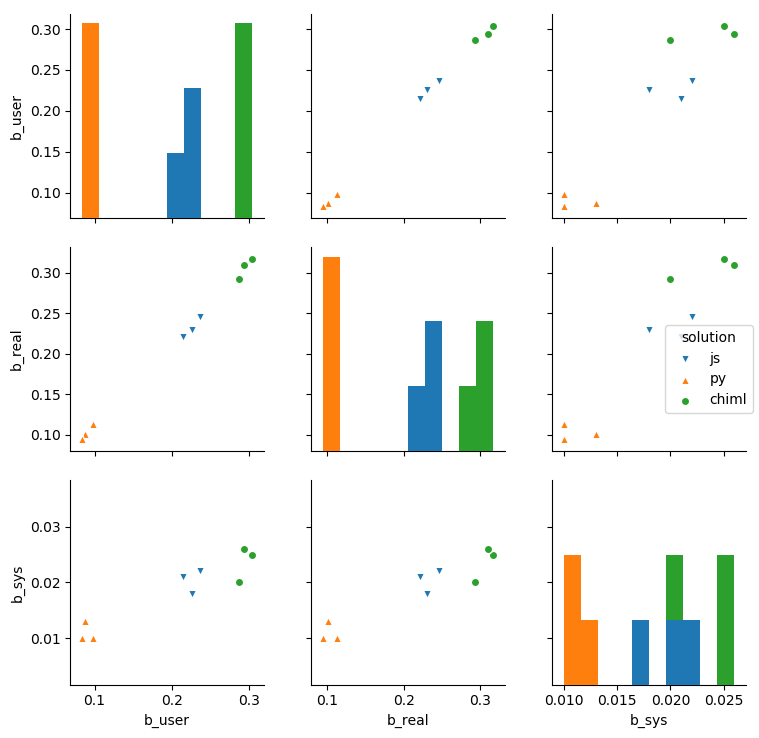
\includegraphics[width=0.5\textwidth]
		{benchmark/benchmark.png}
	\caption{Performance Comparison}
	\label{fig:performanceComparison}
\end{figure*}

\begin{figure*}
	\centering
	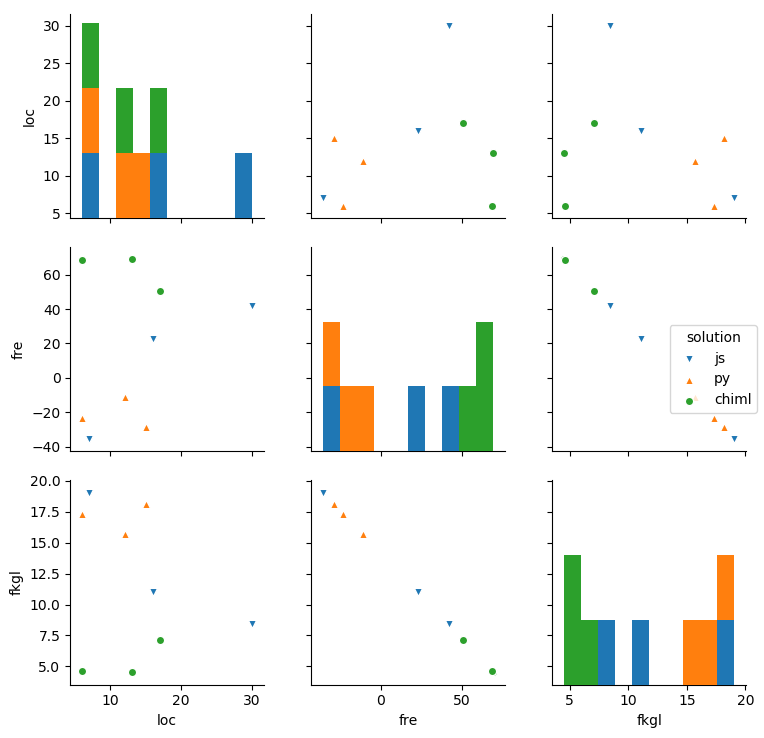
\includegraphics[width=0.7\textwidth]
		{benchmark/readability.png}
	\caption{Readability Comparison}
	\label{fig:readabilityComparison}
\end{figure*}

After building the solutions, we compare the performance by using UNIX {\it time} command. This benchmark providing 3 numbers, {\it sys}, {\it user}, and {\it real}. {\it Sys} is the amount of CPU time spent within kernel. {\it User} is the amount of CPU time spent outside the kernel but within the process. And {\it real} is the clock time from start to finish the call. {\it Real} also include time spent for IO process. We named these performance {\it b\_sys}, {\it b\_real}, and {\it b\_user} respectively.

Beside comparing the performance, we also calculate the file size in byte ({\it size}), number of lines in code ({\it loc}), Flesch reading ease ({\it fre}), and Flesh-Kincaid grade level ({\it fkgl}).

For {\it b\_sys}, {\it b\_real}, and {\it b\_user}, smaller number means better performance. For {\it size} and {\it loc}, smaller number is also means better. For {\it fre}, greater numbers means that the program is more readable. However, for {\it fkgl}, smaller number means smaller years of education required. This means that {\it fkgl} and {\it fre} should has negative correlation.

The result is presented in the table ~\ref{tbl:comparison}.

As shown in figure ~\ref{fig:performanceComparison}, we can conclude that Python solution is unexpectedly outperforming Javascript and CHIML. This is interesting, since in our solutions we didn't use multithread strategy. Python was expected to be slower because it has no non-blocking mechanism by default. However, the experiment show different result.

Also, {\it b\_user} and {\it b\_real} is strongly corelated to each other. This is make sense since the majority CPU time is spent in {\it user} mode.

In term of performance, CHIML solution is the slowest. This is also make sense, since under the hood, CHIML will be translated into JavaScript. 

In terms of {\it size}, CHIML outperforming Python and JavaScript. The same is also true for {\it fkgl} and {\it fre}. Thus, we can conclude that according to Flesch-Kincaid readability test, CHIML is more readable from Python and JavaScript.

CHIML is unexpectedly slow when performing map or filter. It seems to be related to it's internal mechanism in translating map/filter. In CHIML, map and filter is translated into starting another subchain-execution.

We also realize that starting another external process (like UNIX tool) from CHIML is sometime take less time than running JavaScript expression inside CHIML (i.e: we use JavaScript to evaluate control structure). We are still trying to analyze this trait, but there are some possibilities that we have to consider. The first possibility is related to Chimera-Framework mechanism in evaluating JavaScript expression. Since internally we use {\it script.runInNewContext(context)}, the interpreter will always copy global variables and creating new context everytime. When the content of global variables increases, this can drag down the performance. The second possibility is related to Node.Js single thread nature. Eventough internally Node.Js can use more than one processor in a single thread, this will not work for our local code. In some cases, especially when the code doesn't involve IO process, everything will be executed sequentially.

So, for the sake of improving performance, we should refine CHIML parser and interpreter. Either by switching to a more concurrent language like {\it golang}, or by optimizing the current parser and interpreter. One of the possible solutions is using {\it child\_process.fork} that allow us to run the sub-process in other thread.


\section{Conclusion}

CHIML serve well as orchestration language. However for control structure, the existance of intermediary components can help to boost performance. The best trait of CHIML is it's support for programming-in-large and programming-in-small. Eventough the control structure is still suffering for speed and performance, it serves well as prototyping tool. In term of flexibility, CHIML is comparable to Python or JavaScript. In most cases, it even has smallest size and LOC than both, Python and JavaScript. This mean that the developer can start orchestration solution in CHIML, and gradually do optimization as needed.

Despite of it's advantage, CHIML interpreter has to be refactored and optimized in order to make it usable for real-world use-cases.

%\appendices
%\section{Proof of the First Zonklar Equation}

% use section* for acknowledgement
%\section*{Acknowledgment}

%The authors would like to thank Sonny Setiawan, Satriyo Wibowo, Dani Devito, and Zusana Pudyastuti for their suggestions and inputs.

% Can use something like this to put references on a page
% by themselves when using endfloat and the captionsoff option.
\ifCLASSOPTIONcaptionsoff
  \newpage
\fi

\bibliographystyle{IEEEtran}
\bibliography{./citation}

% that's all folks
\end{document}

